\documentclass[journal,12pt,twocolumn]{IEEEtran}
%
\usepackage{setspace}
\usepackage{gensymb}
%\doublespacing
\singlespacing

%\usepackage{graphicx}
%\usepackage{amssymb}
%\usepackage{relsize}
\usepackage[cmex10]{amsmath}
%\usepackage{amsthm}
%\interdisplaylinepenalty=2500
%\savesymbol{iint}
%\usepackage{txfonts}
%\restoresymbol{TXF}{iint}
%\usepackage{wasysym}
\usepackage{amsthm}
\usepackage{iithtlc}
\usepackage{mathrsfs}
\usepackage{txfonts}
\usepackage{stfloats}
\usepackage{bm}
\usepackage{cite}
\usepackage{cases}
\usepackage{subfig}
%\usepackage{xtab}
\usepackage{longtable}
\usepackage{multirow}
%\usepackage{algorithm}
%\usepackage{algpseudocode}
\usepackage{enumitem}
\usepackage{mathtools}
\usepackage{tikz}
\usepackage{circuitikz}
\usepackage{verbatim}
\usepackage{tfrupee}
\usepackage[breaklinks=true]{hyperref}
%\usepackage{stmaryrd}
\usepackage{tkz-euclide} % loads  TikZ and tkz-base
\usetkzobj{all}
\usepackage{listings}
    \usepackage{color}                                            %%
    \usepackage{array}                                            %%
    \usepackage{longtable}                                        %%
    \usepackage{calc}                                             %%
    \usepackage{multirow}                                         %%
    \usepackage{hhline}                                           %%
    \usepackage{ifthen}                                           %%
  %optionally (for landscape tables embedded in another document): %%
    \usepackage{lscape}     
\usepackage{multicol}
\usepackage{chngcntr}
%\usepackage{enumerate}

%\usepackage{wasysym}
%\newcounter{MYtempeqncnt}
\DeclareMathOperator*{\Res}{Res}
%\renewcommand{\baselinestretch}{2}
\renewcommand\thesection{\arabic{section}}
\renewcommand\thesubsection{\thesection.\arabic{subsection}}
\renewcommand\thesubsubsection{\thesubsection.\arabic{subsubsection}}

\renewcommand\thesectiondis{\arabic{section}}
\renewcommand\thesubsectiondis{\thesectiondis.\arabic{subsection}}
\renewcommand\thesubsubsectiondis{\thesubsectiondis.\arabic{subsubsection}}

% correct bad hyphenation here
\hyphenation{op-tical net-works semi-conduc-tor}
\def\inputGnumericTable{}                                 %%

\lstset{
%language=C,
frame=single, 
breaklines=true,
columns=fullflexible
}
%\lstset{
%language=tex,
%frame=single, 
%breaklines=true
%}

\begin{document}
%


\newtheorem{theorem}{Theorem}[section]
\newtheorem{problem}{Problem}
\newtheorem{proposition}{Proposition}[section]
\newtheorem{lemma}{Lemma}[section]
\newtheorem{corollary}[theorem]{Corollary}
\newtheorem{example}{Example}[section]
\newtheorem{definition}[problem]{Definition}
%\newtheorem{thm}{Theorem}[section] 
%\newtheorem{defn}[thm]{Definition}
%\newtheorem{algorithm}{Algorithm}[section]
%\newtheorem{cor}{Corollary}
\newcommand{\BEQA}{\begin{eqnarray}}
\newcommand{\EEQA}{\end{eqnarray}}
\newcommand{\define}{\stackrel{\triangle}{=}}

\bibliographystyle{IEEEtran}
%\bibliographystyle{ieeetr}


\providecommand{\mbf}{\mathbf}
\providecommand{\pr}[1]{\ensuremath{\Pr\left(#1\right)}}
\providecommand{\qfunc}[1]{\ensuremath{Q\left(#1\right)}}
\providecommand{\sbrak}[1]{\ensuremath{{}\left[#1\right]}}
\providecommand{\lsbrak}[1]{\ensuremath{{}\left[#1\right.}}
\providecommand{\rsbrak}[1]{\ensuremath{{}\left.#1\right]}}
\providecommand{\brak}[1]{\ensuremath{\left(#1\right)}}
\providecommand{\lbrak}[1]{\ensuremath{\left(#1\right.}}
\providecommand{\rbrak}[1]{\ensuremath{\left.#1\right)}}
\providecommand{\cbrak}[1]{\ensuremath{\left\{#1\right\}}}
\providecommand{\lcbrak}[1]{\ensuremath{\left\{#1\right.}}
\providecommand{\rcbrak}[1]{\ensuremath{\left.#1\right\}}}
\theoremstyle{remark}
\newtheorem{rem}{Remark}
\newcommand{\sgn}{\mathop{\mathrm{sgn}}}
\providecommand{\abs}[1]{\left\vert#1\right\vert}
\providecommand{\res}[1]{\Res\displaylimits_{#1}} 
\providecommand{\norm}[1]{\left\lVert#1\right\rVert}
%\providecommand{\norm}[1]{\lVert#1\rVert}
\providecommand{\mtx}[1]{\mathbf{#1}}
\providecommand{\mean}[1]{E\left[ #1 \right]}
\providecommand{\fourier}{\overset{\mathcal{F}}{ \rightleftharpoons}}
%\providecommand{\hilbert}{\overset{\mathcal{H}}{ \rightleftharpoons}}
\providecommand{\system}{\overset{\mathcal{H}}{ \longleftrightarrow}}
	%\newcommand{\solution}[2]{\textbf{Solution:}{#1}}
\newcommand{\solution}{\noindent \textbf{Solution: }}
\newcommand{\cosec}{\,\text{cosec}\,}
\providecommand{\dec}[2]{\ensuremath{\overset{#1}{\underset{#2}{\gtrless}}}}
\newcommand{\myvec}[1]{\ensuremath{\begin{pmatrix}#1\end{pmatrix}}}
\newcommand{\mydet}[1]{\ensuremath{\begin{vmatrix}#1\end{vmatrix}}}
%\numberwithin{equation}{section}
\numberwithin{equation}{subsection}
%\numberwithin{problem}{section}
%\numberwithin{definition}{section}
\makeatletter
\@addtoreset{figure}{problem}
\makeatother

\let\StandardTheFigure\thefigure
\let\vec\mathbf
%\renewcommand{\thefigure}{\theproblem.\arabic{figure}}
\renewcommand{\thefigure}{\theproblem}
%\setlist[enumerate,1]{before=\renewcommand\theequation{\theenumi.\arabic{equation}}
%\counterwithin{equation}{enumi}


%\renewcommand{\theequation}{\arabic{subsection}.\arabic{equation}}

\def\putbox#1#2#3{\makebox[0in][l]{\makebox[#1][l]{}\raisebox{\baselineskip}[0in][0in]{\raisebox{#2}[0in][0in]{#3}}}}
     \def\rightbox#1{\makebox[0in][r]{#1}}
     \def\centbox#1{\makebox[0in]{#1}}
     \def\topbox#1{\raisebox{-\baselineskip}[0in][0in]{#1}}
     \def\midbox#1{\raisebox{-0.5\baselineskip}[0in][0in]{#1}}

\vspace{3cm}

\title{
	\logo{
School Arithmetic through  Physics and Chemistry
	}
}
\author{ G V V Sharma$^{*}$% <-this % stops a space
	\thanks{*The author is with the Department
		of Electrical Engineering, Indian Institute of Technology, Hyderabad
		502285 India e-mail:  gadepall@iith.ac.in. All content in this manual is released under GNU GPL.  Free and open source.}
	
}	
%\title{
%	\logo{Matrix Analysis through Octave}{\begin{center}
\includegraphics[scale=.24]{tlc}\end{center}}{}{HAMDSP}
%}


% paper title
% can use linebreaks \\ within to get better formatting as desired
%\title{Matrix Analysis through Octave}
%
%
% author names and IEEE memberships
% note positions of commas and nonbreaking spaces ( ~ ) LaTeX will not break
% a structure at a ~ so this keeps an author's name from being broken across
% two lines.
% use \thanks{} to gain access to the first footnote area
% a separate \thanks must be used for each paragraph as LaTeX2e's \thanks
% was not built to handle multiple paragraphs
%

%\author{<-this % stops a space
%\thanks{}}
%}
% note the % following the last \IEEEmembership and also \thanks - 
% these prevent an unwanted space from occurring between the last author name
% and the end of the author line. i.e., if you had this:
% 
% \author{....lastname \thanks{...} \thanks{...} }
%                     ^------------^------------^----Do not want these spaces!
%
% a space would be appended to the last name and could cause every name on that
% line to be shifted left slightly. This is one of those "LaTeX things". For
% instance, "\textbf{A} \textbf{B}" will typeset as "A B" not "AB". To get
% "AB" then you have to do: "\textbf{A}\textbf{B}"
% \thanks is no different in this regard, so shield the last } of each \thanks
% that ends a line with a % and do not let a space in before the next \thanks.
% Spaces after \IEEEmembership other than the last one are OK (and needed) as
% you are supposed to have spaces between the names. For what it is worth,
% this is a minor point as most people would not even notice if the said evil
% space somehow managed to creep in.



% The paper headers
%\markboth{Journal of \LaTeX\ Class Files,~Vol.~6, No.~1, January~2007}%
%{Shell \MakeLowercase{\textit{et al.}}: Bare Demo of IEEEtran.cls for Journals}
% The only time the second header will appear is for the odd numbered pages
% after the title page when using the twoside option.
% 
% *** Note that you probably will NOT want to include the author's ***
% *** name in the headers of peer review papers.                   ***
% You can use \ifCLASSOPTIONpeerreview for conditional compilation here if
% you desire.




% If you want to put a publisher's ID mark on the page you can do it like
% this:
%\IEEEpubid{0000--0000/00\$00.00~\copyright~2007 IEEE}
% Remember, if you use this you must call \IEEEpubidadjcol in the second
% column for its text to clear the IEEEpubid mark.



% make the title area
\maketitle

\newpage

\tableofcontents

\bigskip

\renewcommand{\thefigure}{\theenumi}
\renewcommand{\thetable}{\theenumi}
%\renewcommand{\theequation}{\theenumi}

%\begin{abstract}
%%\boldmath
%In this letter, an algorithm for evaluating the exact analytical bit error rate  (BER)  for the piecewise linear (PL) combiner for  multiple relays is presented. Previous results were available only for upto three relays. The algorithm is unique in the sense that  the actual mathematical expressions, that are prohibitively large, need not be explicitly obtained. The diversity gain due to multiple relays is shown through plots of the analytical BER, well supported by simulations. 
%
%\end{abstract}
% IEEEtran.cls defaults to using nonbold math in the Abstract.
% This preserves the distinction between vectors and scalars. However,
% if the journal you are submitting to favors bold math in the abstract,
% then you can use LaTeX's standard command \boldmath at the very start
% of the abstract to achieve this. Many IEEE journals frown on math
% in the abstract anyway.

% Note that keywords are not normally used for peerreview papers.
%\begin{IEEEkeywords}
%Cooperative diversity, decode and forward, piecewise linear
%\end{IEEEkeywords}



% For peer review papers, you can put extra information on the cover
% page as needed:
% \ifCLASSOPTIONpeerreview
% \begin{center} \bfseries EDICS Category: 3-BBND \end{center}
% \fi
%
% For peerreview papers, this IEEEtran command inserts a page break and
% creates the second title. It will be ignored for other modes.
%\IEEEpeerreviewmaketitle

\begin{abstract}
This book provides applications of arithmetic using problems from Physics and Chemistry from class 9-12. Links to sample Python codes are available in the text.  
\end{abstract}
Download python codes using 
\begin{lstlisting}
svn co https://github.com/gadepall/school/trunk/ncert/arithmetic/codes
\end{lstlisting}

%\section{Triangle}
%\subsection{Triangle Examples}
%\renewcommand{\theequation}{\theenumi}
\begin{enumerate}[label=\arabic*.,ref=\thesubsection.\theenumi]
\numberwithin{equation}{enumi}
%
\item Do the points $\vec{A}=\myvec{3\\2}, \vec{B}=\myvec{-2\\-3}, \vec{C}=\myvec{2\\3} $ form a triangle?  If so, name the type of triangle formed.
\label{prob:tri_exam_coll_pts}
%
\\
\solution The direction vectors of $AB$ and $BC$ are 
\begin{align}
\label{eq:tri_geo_ex_baorth}
\vec{B}-\vec{A} &= \myvec{-5\\-5}
\\
\vec{C}-\vec{A} &= \myvec{-1\\1}
\label{eq:tri_geo_ex_caorth}
\end{align}
%
Since 
%
\begin{align}
\vec{B}-\vec{A} \ne k\brak{\vec{C}-\vec{A}},
\end{align}
%
the points are not collinear and form a triangle.  An alternative method is to create the matrix
\begin{align}
\label{eq:tri_geo_ex_diff_mat}
\vec{M} = \myvec{\vec{B}-\vec{A} & \vec{B}-\vec{A}}^T 
\end{align}
%
If $rank(\vec{M}) = 1$, the points are collinear.  The rank of a matrix is the number of nonzero rows left after doing row operations.  In this problem, 
%
\begin{align}
\vec{M} = \myvec{-5 & -5\\-1 & 1}\xleftrightarrow {R_2\leftarrow 5R_2-R_1}\myvec{-5 & -5\\0 & 10}
\\
\implies rank(\vec{M}) = 2
\end{align}
%
as the number of non zero rows is 2.
The following code plots Fig. \ref{fig:check_tri}
%
\begin{lstlisting}
codes/triangle/check_tri.py
\end{lstlisting}
%
\begin{figure}[!ht]
\includegraphics[width=\columnwidth]{./triangle/figs/check_tri.eps}
\caption{}
\label{fig:check_tri}
\end{figure}
%
From the figure, it appears that $\triangle ABC$ is right angled, with $BC$ as the hypotenuse.  From Baudhayana's theorem, this would be true if 
\begin{align}
\norm{\vec{B}-\vec{A}}^2+\norm{\vec{C}-\vec{A}}^2&=\norm{\vec{B}-\vec{C}}^2
\end{align}
which, from \eqref{eq:tri_const_norm_ac} can be expressed as
\begin{multline}
\norm{\vec{A}}^2 + \norm{\vec{C}}^2 - 2\vec{A}^T\vec{C}+
\norm{\vec{A}}^2 + \norm{\vec{B}}^2 - 2\vec{A}^T\vec{B}
\\
=
\norm{\vec{B}}^2 + \norm{\vec{C}}^2 - 2\vec{B}^T\vec{C}
\end{multline}
%
to obtain 
\begin{align}
\label{eq:tri_geo_ex_orth}
\brak{\vec{B}-\vec{A}}^T\brak{\vec{C}-\vec{A}}&=0
\end{align}
%
after simplification.  From \eqref{eq:tri_geo_ex_baorth} and \eqref{eq:tri_geo_ex_caorth}, it is easy to verify that 
\begin{align}
\label{eq:tri_geo_ex_orth_sol}
\brak{\vec{B}-\vec{A}}^T\brak{\vec{C}-\vec{A}}=
 \myvec{-5 & -5}\myvec{-1\\1} = 0
\end{align}
satisfying
\eqref{eq:tri_geo_ex_orth}. Thus,  $\triangle ABC$ is right angled at $\vec{A}$.
%
\item Find the area of a triangle whose vertices are 
$\vec{A}=\myvec{1\\-1}, 
\vec{B} = \myvec{-4\\6}$ and
$ 
\vec{C} = \myvec{-3\\-5}
$.
%
\\
\solution In Fig. \ref{fig:rt_triangle}, from Baudhayana's theorem, 
\begin{align}
\label{eq:tri_geo_baudh}
b^2 = a^2+c^2 &
\\
=b^2\cos^2C+b^2\sin^2C &
\\
\implies \cos^2C+\sin^2C &= 1
\end{align}
%
In Fig. \ref{fig:tri_const_ex_cos_form}, the area of $\triangle ABC$ is defined as
{\footnotesize
\begin{align}
\label{eq:tri_geo_area_sin_form}
\frac{1}{2}ah &= \frac{1}{2}ab\sin C
\\
&=\frac{1}{2}ab\sqrt{1-\cos^2C} \quad \brak{\text{from } \eqref{eq:tri_geo_baudh}
}
\\
&=\frac{1}{2}ab\sqrt{1-\brak{\frac{a^2+b^2-c^2}{2ab}}^2} \brak{\text{from } \eqref{eq:cosC}
}
\\
&=\frac{1}{4}\sqrt{\brak{2ab}^2-\brak{a^2+b^2-c^2}}
\\
&=\frac{1}{4}\sqrt{\brak{2ab+a^2+b^2-c^2}\brak{2ab-a^2-b^2+c^2}}
\\
&= \frac{1}{4}\sqrt{\cbrak{\brak{a+b}^2-c^2}\cbrak{c^2-\brak{a-b}^2}}
\\
&= \frac{1}{4}\sqrt{\brak{a+b+c}\brak{a+b-c}\brak{a+c-b}\brak{b+c-a}}
\label{eq:tri_ex_hero_temp}
\end{align}
}
Substituting 
%
\begin{align}
s=\frac{a+b+c}{2}
\end{align}
%
in \eqref{eq:tri_ex_hero_temp}, the area of $\triangle ABC$ is 
%
\begin{align}
\sqrt{s\brak{s-a}\brak{s-b}\brak{s-c}}
\end{align}
%
This is known as Hero's formula.  The following code computes the area of the  triangle as 24.
%
\begin{lstlisting}
codes/triangle/area_tri.py
\end{lstlisting}
%
%
\item Find the area of a triangle formed by the vertices $\vec{A}=\myvec{5\\2}, \vec{B}=\myvec{4\\7}, \vec{C}=\myvec{7\\-4}$.
\\
\solution  The area of $\triangle ABC$ is also obtained  in terms of the  {\em magnitude} of the determinant of the matrix $\vec{M}$ in  \eqref{eq:tri_geo_ex_diff_mat} as
%
\begin{align}
\frac{1}{2}\mydet{\vec{M}}
\end{align}
The computation is done in \textbf{area\_tri.py}
\item Find the area of a triangle formed by the points $\vec{P}=\myvec{-1.5\\3}, \vec{Q}=\myvec{6\\-2}, \vec{R}=\myvec{-3\\4}$.
\\
\solution Another formula for the area of $\triangle ABC$  is
%
\begin{align}
\frac{1}{2}\mydet{1 & 1 & 1\\ \vec{A} & \vec{B} & \vec{C} }
\end{align}
%
\item Find the area of a triangle having the points
%
\begin{align}
\vec{A} = \myvec{1\\1 \\1},
\vec{B} = \myvec{1\\2 \\3},
\vec{C} = \myvec{2\\ 3\\1}
\end{align}
%
as its vertices.
\\
\solution The area of a triangle using the {\em vector product} is obtained as
\begin{align}
\frac{1}{2}\norm{\brak{\vec{B}-\vec{A}}\times \brak{\vec{C}-\vec{A}}}
\end{align}
%
For any two vectors $\vec{a}=\myvec{a_1\\a_2\\a_3}, \vec{b}=\myvec{b_1\\b_2\\b_3}$, 
\begin{align}
\label{eq:tri_cross_prod}
\vec{a}\times \vec{b} = \myvec{0 & -a_3 & a_2 \\ a_3 & 0 & -a_1 \\ -a_2 & a_1 & 0}\myvec{b_1\\b_2\\b_3}
\end{align}
%
The following code computes the area using the vector product.
%
\begin{lstlisting}
codes/triangle/area_tri_vec.py
\end{lstlisting}
%
%
\item The centroid of a $\triangle ABC$ is at the point \myvec{1\\1\\1}.  If the coordinates of $\vec{A}$ and $\vec{B}$ are \myvec{3\\-5\\7} and \myvec{-1\\7\\-6}, respectively, find the coordinates of the point $\vec{C}$.
%
\\
\solution The centroid of $\triangle ABC$ is given by
\begin{align}
\label{eq:tri_geo_ex_centroid}
\vec{O} = \frac{\vec{A}+\vec{B}+\vec{C}}{3}
\end{align}
%
Thus, 
\begin{align}
\vec{C} = 3\vec{C}-\vec{A}-\vec{B}
\end{align}
%
\item Show that the points 
\begin{align}
\vec{A} = \myvec{2\\-1 \\1},
\vec{B} = \myvec{1\\-3 \\-5},
\vec{C} = \myvec{3\\ -4\\-4}
\end{align}
%
are the vertices of a right angled triangle.
\\
\solution 
The following code plots Fig. \ref{fig:triangle_3d}
%
\begin{lstlisting}
codes/triangle/triangle_3d.py
\end{lstlisting}
%
\begin{figure}[!ht]
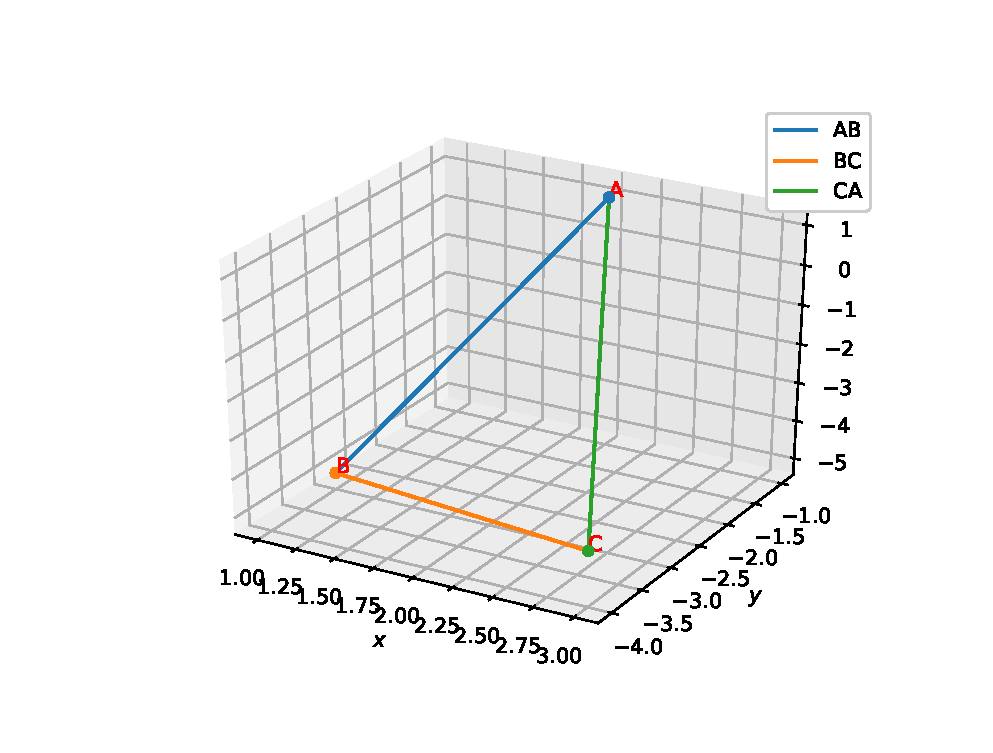
\includegraphics[width=\columnwidth]{./triangle/figs/triangle_3d.eps}
\caption{}
\label{fig:triangle_3d}
\end{figure}
%
From the figure, it appears that $\triangle ABC$ is right angled at $\vec{C}$.  Since 
\begin{align}
\brak{\vec{A}-\vec{C}}^T\brak{\vec{B}-\vec{C}}&=0
\end{align}
%
it is proved that the triangle is indeed right angled.
 \item Are the points 
\begin{align}
\vec{A} = \myvec{3\\6 \\9},
\vec{B} = \myvec{10\\20 \\30},
\vec{C} = \myvec{25\\ -41\\5},
\end{align}
%
the vertices of a right angled triangle?
%
\item A tower stands vertically on the ground.  From a point on the ground, which is 15m away from the foot of the tower, the angle of elevation of the top of the tower is found to be 60$\degree$.  Find the height of the tower.
%
\begin{figure}[!ht]
\includegraphics[width=\columnwidth]{./triangle/figs/Trig/pg1.eps}
\caption{}
\label{fig:trig_pg1}
\end{figure}
%
\\
\solution Fig. \ref{fig:trig_pg1} summarizes the problem. 
%
\begin{align}
h = b\tan\theta = 15\tan60\degree = 15\sqrt{3}
\end{align}
%
\item An electrician has to repair an electric fault pole of height 5m.  She needs to reach a point 1.3m below the top of the pole to undertake the repair work.  What should be the length of the ladder that she should use which, when inclined at an angle of 60$\degree$ to the horizontal, would enable her to reach the required position?  Also, how far from the foot of the pole should she place the foot of the ladder?
%
\begin{figure}[!ht]
\includegraphics[width=\columnwidth]{./triangle/figs/Trig/pg2.eps}
\caption{}
\label{fig:trig_pg2}
\end{figure}
%
\\
\solution Fig. \ref{fig:trig_pg2} summarizes the problem. The objective is to find $l$ and $b$.  From the figure,
%
if 
\begin{align}
\cot \theta &=\frac{1}{\tan \theta},
\\
h-x &= l\sin \theta = b\tan \theta
\\
\implies l &= \brak{h-x}\csc \theta = 3.7\csc60\degree 
\\
\text{and } b&=\brak{h-x}\cot\theta = 3.7 \cot \degree 
\end{align}
\item An observer 1.5m tall is 28.5m away from a chimney.  The angle of elevation of the top of the chimney from her eyes is 45$\degree$.  What is the height of the chimney?
%
%
\begin{figure}[!ht]
\includegraphics[width=\columnwidth]{./triangle/figs/Trig/pg3.eps}
\caption{}
\label{fig:trig_pg3}
\end{figure}
%
\\
\solution Fig. \ref{fig:trig_pg3} summarizes the problem. The objective is to find $h$.  From the figure,
%
\begin{align}
h-h_1 &=  b\tan \theta
\\
\implies h &= h_1+b\tan\theta 
\\
&= 1.5+28.5\tan45\degree 
\\
&= 30m
\end{align}
\item From a point $\vec{P}$ on the ground the angle of elevation of the top of a 10m tall building is 30$\degree$.  A flag is hoisted at the top of the building and the angle of elevation of the top of the flagstaff from $\vec{P}$ is $45\degree$.  Find the length of the flagstaff and the distance of the building from the point $\vec{P}$.
%
\begin{figure}[!ht]
\includegraphics[width=\columnwidth]{./triangle/figs/Trig/pg4.eps}
\caption{}
\label{fig:trig_pg4}
\end{figure}
%
\\
\solution Fig. \ref{fig:trig_pg4} summarizes the problem. The objective is to find $h_2$ and $b$ while $h_1$ is known.  From the figure, 
%
\begin{align}
h_1+h_2 &=  b\tan \theta_1
\\
h_1 &= b\tan \theta_2
\end{align}
%
This can be expressed as the matrix equation 
%
\begin{align}
\myvec{
\tan \theta_1 & -1
\\
\tan \theta_2 &0
}\myvec{b\\h_2}
= h_1\myvec{1\\1}
\end{align}
%
and solved.
\item The shadow of a tower standing on a level ground is found to be 40m longer when the Sun's altitude is 30$\degree$ than when it is $60\degree$.  Find the height of the tower.
%
\begin{figure}[!ht]
\includegraphics[width=\columnwidth]{./triangle/figs/Trig/pg5.eps}
\caption{}
\label{fig:trig_pg5}
\end{figure}
%
\\
\solution Fig. \ref{fig:trig_pg5} summarizes the problem. The objective is to find $h$.  from the figure,
%
\begin{align}
b_1 &= h\cot 60\degree
\\
b_2 &= h\cot 30\degree
\\
b_2-b_1 &= 40
\\
\implies h \brak{\cot 30\degree-\cot 60\degree}&= 40
\\
\text{or } h &= \frac{40}{\cot 30\degree-\cot 60\degree}
\end{align}
%
\item The angles of depression of the top and the bottom of an 8m tall building from the top of a multi-storeyed building are 30$\degree$ and 45$\degree$ respectively.  Find the height of the multi-storeyed building and the distance between the two buildings.
%
\begin{figure}[!ht]
\includegraphics[width=\columnwidth]{./triangle/figs/Trig/pg6.eps}
\caption{}
\label{fig:trig_pg6}
\end{figure}
%
\\
\solution Fig. \ref{fig:trig_pg6} summarizes the problem. The objective is to find $h_2$ and $b$.  From the figure, 
%
\begin{align}
h_2 &= b\tan \theta_2
\\
h_2-h_1 &= b\tan \theta_1
\end{align}
%
which can be expressed as
%
\begin{align}
\myvec{
 1 & -\tan\theta_2 
\\
 1 & -\tan\theta_1
}\myvec{h_2\\b}
= h_1\myvec{0\\1}
\end{align}
%
and solved.
\end{enumerate}
%
 
%\subsection{Triangle Exercises}
%\renewcommand{\theequation}{\theenumi}
\begin{enumerate}[label=\arabic*.,ref=\thesubsection.\theenumi]
\numberwithin{equation}{enumi}
%
\item Draw the graphs of the equations 
\begin{align}
\myvec{1 & -1}\vec{x} + 1 &= 0 
\\
\myvec{ 3 & 2} - 12 &= 0
\end{align}
%
 Determine the coordinates of the vertices of the triangle formed by these lines and the x-axis, and shade the triangular region.
%
\item The vertices of $\triangle PQR$ are 

$
\vec{P} = \myvec{2 \\1},
\vec{Q} = \myvec{-2\\3},
\vec{R} = \myvec{4\\5}.
$
Find the equation of the median through the vertex $\vec{R}$.
\item In the $\triangle ABC$ with vertices
$
\vec{A}=\myvec{2\\3}, 
\vec{B}=\myvec{4\\-1},
 \vec{C}=\myvec{1\\2}
$,
find the equation and length of the altitude from the vertex $\vec{A}$.
\item Find the area of the triangle whose vertices are
\begin{enumerate}
\item \myvec{2\\3}, \myvec{-1\\0},  \myvec{2\\-4}
\item  \myvec{-5\\-1},  \myvec{3\\-5},  \myvec{5\\2}
\end{enumerate}
\item Find the area of the triangle formed by joining the mid points o the sides of a triangle whose vertices are  \myvec{0\\-1},  \myvec{2\\1},  \myvec{0\\3}.
\item Verify that the median of $\triangle ABC$ with vertices $\vec{A}=\myvec{4\\-6},  \vec{B}=\myvec{3\\-2}$ and  $\vec{C} =  \myvec{5\\2}$ divides it into two triangles of equal areas.
\item The vertices of $\triangle ABC$ are $\vec{A}=\myvec{4\\6},  \vec{B}=\myvec{1\\5}$ and  $\vec{C} =  \myvec{7\\2}$.  A line is drawn to intersect sides $AB$ and $AC$ at $D$ and $E$ respectively, such that
\begin{align}
\frac{AD}{AB}=\frac{AE}{AC}= \frac{1}{4}
\end{align}
%
Find 
\begin{align}
\frac{\text{area of }\triangle ADE}{\text{area of }\triangle ABC}.
\end{align}
\item Let $\vec{A}=\myvec{4\\2},  \vec{B}=\myvec{6\\5}$ and  $\vec{C} =  \myvec{1\\4}$ be the vertices of $\triangle ABC$.
\begin{enumerate}
\item The median from $\vec{A}$ meets $BC$ at $\vec{D}$.  Find the coordinates of the point $\vec{D}$.
\item Find the coordinates of the point $\vec{P}$ on $AD$ such that $AP:PD = 2:1$.
\item Find the coordinates of the points $\vec{Q}$ and $\vec{R}$ on medians $BE$ and $CF$ respectively such that $BQ:QE = 2:1$ and $CR:RF = 2:1$.
\end{enumerate}
\item In $\triangle ABC$, Show that the centroid 
\begin{align}
\vec{O} = \frac{\vec{A}+\vec{B}+\vec{C}}{3}
\end{align}
\item Show that the points 
\begin{align}
\vec{A} = \myvec{2\\-1 \\1},
\vec{B} = \myvec{1\\-3 \\-5},
\vec{C} = \myvec{3\\ -4\\-4}
\end{align}
%
are the vertices of a right angled triangle.
\item In $\triangle ABC$, 
$
\vec{A} = \myvec{1\\2 \\3},
\vec{B} = \myvec{-1\\0 \\0},
\vec{C} = \myvec{0\\ 1\\2}.
$
Find $\angle B$.
\item Show that the vectors 
$
\myvec{2\\-1 \\1},
\myvec{1\\-3 \\-5},
\myvec{3\\ -4\\-4}
$
form the vertices of a right angled triangle.
\item Find the area of a triangle having the points 
$
\vec{A} = \myvec{1\\1 \\1},
\vec{B} = \myvec{1\\2 \\3}, \text{ and }
\vec{C} = \myvec{2\\ 3\\1}
$
as its vertices.
\item Find the area of a triangle with vertices
$
\vec{A} = \myvec{1\\1 \\2},
\vec{B} = \myvec{2\\3 \\5}, \text{ and }
\vec{C} = \myvec{1\\ 5\\5}
$
\item A girl walks 4km west, then she walks 3km in a direction $30\degree$ east of north and stops.  Determine the girl's displacement from her initial point of departure.
\item Find the direction vectors of the sides of a triangle with vertices
$
\vec{A} = \myvec{3\\5 \\-4},
\vec{B} = \myvec{-1\\1 \\2}, \text{ and }
\vec{C} = \myvec{-5\\ -5\\-2}
$
\item Without using the Pythagoras theorem, show that the points \myvec{4\\ 4}, \myvec{3\\ 5} and \myvec{–1\\ –1} are the vertices of a right angled triangle.
\item Check whether 
\begin{align}
\myvec{5\\-2}, \myvec{6\\4}, \myvec{7\\-2}
\end{align}
are the vertices of an isosceles triangle.
%
\item A circus artist is climbing a 20m long rope, which is tightly stretched and tied from the top of a vertical pole to the ground.  Find the height of the pole, if the angle made by the rope with the ground level is 30$\degree$.
%
\item A tree breaks due to storm and the broken part bends so that the top of the tree touches the ground making an angle of 30$\degree$ with it.  The distance between the foot of the tree to the point where the top touches the ground is 8m.  Find the height of the tree.
%
\item A contractor plans to install two slides for the children to play in a park.  For the children below the age of 5 years, she prefers to have a slide whose top is at a height of 1.5m, and is inclined at an angle of 30$\degree$  to the ground, whereas for elder children she wants to have a steep slide at a height of 3m, and inclined at an angle of 60$\degree$ to the ground.  What should be the length of the slide in each case?
%
\item The angle of elevation of the top of a tower from a point on the ground, which is 30m away from the foot of the tower, is 30$\degree$.  Find the height of the tower.
%
\item A kite is flying at a height of 60m above the ground.  The string attached to the kite is temporarily tied to a point on the ground.  The inclination of the string with the ground is $60\degree$.  Find the length of the string, assuming that there is no slack in the string.
%
\item A 1.5m tall boy is standing at some distance from a 30m tall building.  The angle of elevation from his eyes to the top of the building increases from 30$\degree$
 to 60$\degree $ as he walks towards the building.  Find the distance he walked towards the building.

\item From a point on the ground, the angles of elevation of the bottom and the top of a transmission tower fixed at the top of a 20 m high building are 45$\degree$ and 60$\degree$ respectively. Find the height of the tower.

\item A statue, 1.6 m tall, stands on the top of a pedestal. From a point on the ground, the angle of elevation of the top of the statue is 60$\degree$ and from the same point the angle of elevation of the top of the pedestal is 45$\degree$. Find the height of the pedestal.
\item The angle of elevation of the top of a building from the foot of the tower is 30$\degree$ and the angle of elevation of the top of the tower from the foot of the building is 60$\degree$. If the tower is 50 m high, find the height of the building.
\item Two poles of equal heights are standing opposite each other on either side of the road, which is 80 m wide. From a point between them on the road, the angles of elevation of the top of the poles are 60$\degree$ and 30$\degree$, respectively. Find the height of the poles and the distances of the point from the poles.
\item A TV tower stands vertically on a bank of a canal. From a point on the other bank directly opposite the tower, the angle of elevation of the top of the tower is 60$\degree$. From another point 20 m away from this point on the line joing this point to the foot of the tower, the angle of elevation of the top of the tower is 30$\degree$. Find the height of the tower and the width of the canal.
\item From the top of a 7 m high building, the angle of elevation of the top of a cable tower is 60$\degree$ and the angle of depression of its foot is 45$\degree$. Determine the height of the tower.
\item As observed from the top of a 75 m high lighthouse from the sea-level, the angles of depression of two ships are 30$\degree$ and 45$\degree$. If one ship is exactly behind the other on the same side of the lighthouse, find the distance between the two ships.
\item A 1.2 m tall girl spots a balloon moving with the wind in a horizontal line at a height of 88.2 m from the ground. The angle of elevation of the balloon from the eyes of the girl at any instant is 60$\degree$. After some time, the angle of elevation reduces to 30$\degree$. Find the distance travelled by the balloon during the interval.
\item A straight highway leads to the foot of a tower. A man standing at the top of the tower observes a car at an angle of depression of 30$\degree$, which is approaching the foot of the tower with a uniform speed. Six seconds later, the angle of depression of the car is found to be 60$\degree$. Find the time taken by the car to reach the foot of the tower from this point.
\item The angles of elevation of the top of a tower from two points at a distance of 4 m and 9 m from the base of the tower and in the same straight line with it are complementary. Prove that the height of the tower is 6 m.

\end{enumerate}
%

 
%%
%\section{Quadrilateral}
%\subsection{Quadrilateral Examples}
%\renewcommand{\theequation}{\theenumi}
\begin{enumerate}[label=\arabic*.,ref=\thesubsection.\theenumi]
\numberwithin{equation}{enumi}
%
\item Sum of the angles of a quadrilateral is 360$\degree$. 
\\
\solution Draw the diagonal and use the fact that sum of the angles of a triangle is 180$\degree$.
\item  A diagonal of a parallelogram divides it into two congruent triangles. 
\\
\solution The alternate angles for the parallel sides are equal.  The diagonal is common.  Use ASA congruence.
%
\item  In a parallelogram, 
\begin{enumerate}
\item opposite sides are equal 
\item  opposite angles are equal
\item  diagonals bisect each other
\end{enumerate}
%
\solution Since the diagonal divides the parallelogram into two congruent triangles, all the above results follow.
%
\item  A quadrilateral is a parallelogram, if 
%
\begin{enumerate}
\item opposite sides are equal or 
\item  opposite angles are equal or 
\item  diagonals bisect each other or 
\item a pair of opposite sides is equal and parallel
\end{enumerate}
%
\solution All the above lead to a quadrilateral that has two parallel sides, by showing that the alternate angles are equal.
%
%
\item A rectangle is a parallelogram with one angle that is 90$\degree$.  Show that all angles of the rectangle are 90$\degree$.
%
\\
\solution Draw a diagonal.  Since the diagonal divides the rectangle into two congruent triangles, the angle opposite to the right angle is also 90$\degree$. Using congruence, it can be shown that the other two angles are equal.  Now use the fact that the sum of the angles of a quadrilateral is 360$\degree$.
%
\item  Diagonals of a rectangle bisect each other and are equal and vice-versa. 
%
\\
\solution Use Baudhayana's theorem for equality of diagonals.
%
\item  Diagonals of a rhombus bisect each other at right angles and vice-versa. 
%
\\
\solution The median of an isoceles triangle is also its perpendicular bisector.
%
\item  Diagonals of a square bisect each other at right angles and are equal, and vice-versa. 
%
\\
\solution A square has the properties of a rectangle as well as a rhombus.
%
\item  The line-segment joining the mid-points of any two sides of a triangle is parallel to the third side and is half of it.
\label{prob:quad_similar}
%
\\
\solution If $DE$ is the lie joining he mid points of $\triangle ABC$,  use cosine formula to find the lengths of $DE$ and $BC$. Then use cosine formula to show that all angles of $\triangle ADE$ are equal to the corresponding angles of $\triangle ABC$.
%
\item  A line through the mid-point of a side of a triangle parallel to another side bisects the third side.
\\
\solution Use cosine formula.
%
\item  The quadrilateral formed by joining the mid-points of the sides of a quadrilateral, in order, is a parallelogram.
%
\\
\solution Draw one diagonal and use Problem \eqref{prob:quad_similar}.  Repeat for the other diagonal to show that the sides are parallel.
%
\item Two parallel lines l and m are intersected by a transversal p. Show that the quadrilateral formed by the bisectors of interior angles is a rectangle.
%
\item Show that the bisectors of angles of a parallelogram form a rectangle.
%
\item A quadrilateral is a parallelogram if a pair of opposite sides is equal and parallel.
%
\item $ABCD$ is a parallelogram in which $P$ and $Q$ are mid-points of opposite sides $AB$ and $CD$. If $AQ$ intersects $DP$ at $S$ and $BQ$ intersects $CP$ at $R$, show that: 
%
\begin{enumerate}
\item  $APCQ$ is a parallelogram. 
\item $DPBQ$ is a parallelogram. 
\item $PSQR$ is a parallelogram.
\end{enumerate}
%
\item In $\triangle ABC, D, E$ and $F$ are respectively the mid-points of sides $AB, BC$ and $CA $. Show that $\triangle ABC$ is divided into four congruent triangles by joining $D, E$ and $F$.
\item $l, m$ and $n$ are three parallel lines intersected by transversals $p$ and $q$ such that $l, m$ and $n$ cut off equal intercepts $AB$ and $BC$ on $p$ . Show that $l, m$ and $n$ cut off equal intercepts $DE$ and $EF$ on $q$ also.
%

\item Show that the points $\vec{A} = \myvec{1\\7}, \vec{B} = \myvec{4\\2}, \vec{C}=\myvec{-1\\-1},\vec{D}= \myvec{-4\\4} $  are the vertices of a square.
\\
\solution By inspection, 
%
\begin{align}
\frac{\vec{A}+\vec{C}}{2}=\frac{\vec{B}+\vec{D}}{2} = \myvec{0\\3}
\end{align}
%
Hence, the diagonals $AC$ and $BD$ bisect each other.
%
Also, 
\begin{align}
\brak{\vec{A}-\vec{C}}^T
\brak{\vec{B}-\vec{D}} = 0
\end{align}
%
$\implies AC \perp BD $.  Hence $ABCD$ is a square.
\item If the points
$
\vec{A} = \myvec{6\\1}, 
\vec{B} = \myvec{8\\2}, 
\vec{C} = \myvec{9\\4}, 
\vec{D} = \myvec{p\\3}
$
are the vertices of a parallelogram, taken in order, find the value of $p$.
\\
\solution In the parallelogram $ABCD$, $AC$ and $BD$ bisect each other.  This can be used to find $p$.
\item If $\vec{A} = \myvec{-5\\7}, \vec{B} = \myvec{-4\\-5}, \vec{C} = \myvec{-1\\-6}, \vec{D} = \myvec{4\\5}$, find the area of the quadrilateral $ABCD$.
%
\\
\solution The area of  $ABCD$ is the sum of the areas of trianges ABD and CBD and is given by 
\begin{multline}
\frac{1}{2}\norm{\brak{\vec{A}-\vec{B}}\times \brak{\vec{A}-\vec{D}}}
\\
+
\frac{1}{2}\norm{\brak{\vec{C}-\vec{B}}\times \brak{\vec{C}-\vec{D}}}
\end{multline}
\item Show that the points 
$\vec{A} = \myvec{1\\2\\3},
 \vec{B} = \myvec{-1\\-2\\-1},
\vec{C} = \myvec{2\\3\\2},
\vec{D} = \myvec{4\\7\\6}.
$
are the vertices of a parallelogram $ABCD$ but it is not a rectangle.
%
\\
\solution Since the direction vectors
%
\begin{align}
\vec{A}-\vec{B}&= \vec{D}-\vec{C}
\\
\vec{A}-\vec{D}&= \vec{B}-\vec{C}
\end{align}
%
$AB \parallel CD$ and $AD \parallel BC$.  Hence $ABCD$ is a parallelogram.  However, 
%
\begin{align}
\brak{\vec{A}-\vec{B}}^T\brak{ \vec{A}-\vec{D}}\ne 0
\end{align}
%
Hence, it is not a rectangle.
The following code plots Fig. \ref{fig:quad_3d}
%
\begin{lstlisting}
codes/triangle/quad_3d.py
\end{lstlisting}
%
\begin{figure}[!ht]
\includegraphics[width=\columnwidth]{./triangle/figs/quad_3d.eps}
\caption{}
\label{fig:quad_3d}
\end{figure}
%

\item Find the area of a parallelogram whose adjacent sides are given by the vectors \myvec{3\\1\\4} and \myvec{1\\-1\\1}.
%
\\
\solution  The area is given by 
%
\begin{align}
\frac{1}{2}\norm{\myvec{3\\1\\4} \times \myvec{1\\-1\\1}}
\end{align}
%
\item Kamla has a triangular field with sides 240 m, 200 m, 360 m, where she grew wheat. In another triangular field with sides 240 m, 320 m, 400 m adjacent to the previous field, she wanted to grow potatoes and onions. She divided the field in two parts by joining the mid-point of the longest side to the opposite vertex and grew patatoes in one part and onions in the other part. Draw the figure for this problem.  How much area (in hectares) has been used for wheat, potatoes and onions? (1 hectare = 10000 $m^2$).
\item Students of a school staged a rally for cleanliness campaign. They walked through the lanes in two groups. One group walked through the lanes AB, BC and CA; while the other through AC, CD and DA. Then they cleaned the area enclosed within their lanes. If AB = 9 m, BC = 40 m, CD = 15 m, DA = 28 m and $\angle B = 90\degree$, which group cleaned more area and by how much? Draw the corresponding figure.  Find the total area cleaned by the students (neglecting the width of the lanes). 
%
\item Sanya has a piece of land which is in the shape of a rhombus. She wants her one daughter and one son to work on the land and produce different crops. She divided the land in two equal parts. If the perimeter of the land is 400 m and one of the diagonals is 160 m, how much area each of them will get for their crops? Draw the rhombus.
\end{enumerate}
%
 
%\subsection{Quadrilateral Geometry}
%\renewcommand{\theequation}{\theenumi}
\begin{enumerate}[label=\arabic*.,ref=\thesubsection.\theenumi]
\numberwithin{equation}{enumi}

\item Draw a quadrilateral in the Cartesian plane, whose vertices are \myvec{– 4\\ 5}, \myvec{0\\ 7}, \myvec{5\\ – 5} and \myvec{– 4\\ –2}. Also, find its area.
\item Find the area of a rhombus if its vertices are \myvec{3\\0}, \myvec{4\\5}, \myvec{-1\\4} and \myvec{-2\\-1} taken in order.
\item Without using distance formula, show that points \myvec{– 2\\ – 1}, \myvec{4\\ 0}, \myvec{3\\ 3} and \myvec{–3\\ 2} are the vertices of a parallelogram.
\item  Find the area of the quadrilateral whose vertices, taken in order, are 
 \myvec{-4\\2},  \myvec{-3\\-5},  \myvec{3\\-2},  \myvec{2\\3}. 
\item The two opposite vertices of a square are \myvec{-1\\2},  \myvec{3\\2}. Find the coordinates of the other two vertices.
\item $ABCD$ is a rectangle formed by the points $\vec{A} = \myvec{-1\\-1}, \vec{B} = \myvec{-1\\4}, \vec{C} = \myvec{5\\4}, \vec{D} = \myvec{5\\-1}$. $ \vec{P}, \vec{Q}, \vec{R}, \vec{S}$ are the mid points of $AB, BC, CD, DA$ respectively.  Is the quadrilateral $PQRS$ a 
\begin{enumerate}
\item square?
\item rectangle?
\item rhombus?
\end{enumerate}
\item Find the area of a parallelogram whose adjacent sides are given by the vectors \myvec{3\\1\\4} and \myvec{1\\-1\\1}.
\item Find the area of a parallelogram whose adjacent sides are determined by the vectors $\vec{a} = \myvec{1\\-1\\3}$ and $\vec{b}=\myvec{2\\-7\\1}$.
\item Find the area of a rectangle $ABCD$ with vertices
$\vec{A} = \myvec{-1\\\frac{1}{2}\\ 4},
 \vec{B} = \myvec{1\\\frac{1}{2}\\ 4},
\vec{C} = \myvec{1\\-\frac{1}{2}\\ 4},
\vec{D} = \myvec{-1\\-\frac{1}{2}\\ 4}.
$
\item The two adjacent sides of a parallelogram are \myvec{2\\ -4 \\ -5} and  \myvec{1\\-2\\ -3}. Find the unit vector parallel to its diagonal.  Also, find its area.
\end{enumerate}
%
 
%
\section{Examples}
%\subsection{Equality Constraint}
\renewcommand{\theequation}{\theenumi}
\begin{enumerate}[label=\arabic*.,ref=\thesection.\theenumi]
\numberwithin{equation}{enumi}
%
%
\item An object travels 16m in 4s and then another 16 m in 2 s. What is the average speed of the object?
\item The odometer of a car reads 2000 km at the start of a tri and 2400 km at the end of the trip.  If the trip took 8 h, calculat the average speed of the car in km/h and m/s.
\item Usha swims in a 90m long pool.  She covers 180m in one minute by swimming from one end to the other and back along the same straight path.  Find the average speed and average velocity of Usha.
\item Starting from a stationary position, Rahul paddles his bicycle to
attain a velocity of $6 m s^{-1}$ in $30 s$. Then
he applies brakes such that the velocity of the bicycle comes down to $4 m s^{-1}$
the next $5 s$. Calculate the acceleration of the bicycle in both the cases
%
\item A train starting from rest attains a velocity of $72 km h^{-1}$
in
5 minutes. Assuming that the acceleration is uniform, find (i) the acceleration and (ii) the distance travelled by the train for attaining this velocity.
%
\item A car accelerates uniformly from $18 km h
^{-1}$ to $36 km h^{-1}$ in $5 s$. 
Calculate 
\begin{enumerate}
\item the acceleration and 
\item  the distance covered by the car in that time.
\end{enumerate}
%
\item The brakes applied to a car produce an acceleration of $6 m s^{-2}$
in
the opposite direction to the motion. If the car takes $2 s$ to stop after the application of brakes, calculate the distance it travels during this time.
%
\item A constant force acts on an object of mass 5 kg for a duration of 2 s. It increases the object’s velocity from 3 $m s^{-1}$
to 7 $m s^{-1}$ . Find the
magnitude of the applied force. Now, if the force was applied for a duration of 5 s, what would be the final velocity of the object?
\item Which would require a greater force -- accelerating a 2 kg mass at 5 $m s^{-2}$
or a 4 kg mass at 2 $m s^{-2}$?
\item A motorcar is moving with a velocity of 108 km/h and it takes 4 s to stop after the brakes are applied. Calculate the force exerted by the brakes on the motorcar if its mass along with the passengers is 1000 kg.
\item A force of 5 N gives a mass m1
, an acceleration of 10 $m s^{-2}$ mass m2, an acceleration of 20 $m s^{-2}$
and a .
What acceleration would it give if both the masses were tied together?
\item A bullet of mass 20 g is horizontally fired with a velocity 150 $m s^{-1}$
What is the recoil velocity of the pistol?
\item A girl of mass 40 kg jumps with a horizontal velocity of 5 $m s^{-1}$
onto
a stationary cart with frictionless wheels. The mass of the cart is 3 kg. What is her velocity as the cart starts moving? Assume that there is no external unbalanced force working in the horizontal direction.
\item Two hockey players of opposite teams, while trying to hit a hockey ball on the ground collide and immediately become entangled. One has a mass of 60 kg and was moving with a velocity 5.0 $m s^{-1}$
while the other
has a mass of 55 kg and was moving faster with a velocity 6.0 $m s^{-1}$
towards
the first player. In which direction and with what velocity will they move after they become entangled? Assume that the frictional force acting between the feet of the two players and ground is negligible.

\item The mass of the earth is 6 $\times$ 1024
kg. If the distance between the earth and the moon is 3.84$\times$105
7.4 $\times$ 1022
calculate the force exerted by the earth on the moon. (Take G = 6.7 $\times 10^{-11}
N m^2$ 
\item A car falls off a ledge and drops to the ground in 0.5 s. 
\begin{enumerate}
\item  What is its speed on striking the ground?
\item  What is its average speed during the 0.5 s?
\item  How high is the ledge from the ground?
\end{enumerate}
Let $g = 10 m s^{-2}$.
\item An object is thrown vertically upwards and rises to a height of 10 m. Calculate (i) the velocity with which the object was thrown upwards and (ii) the time taken by the object to reach the highest point. Let $g = 9.8 m s^{-2}$.
\item Mass of an object is 10 kg. What is its weight on the earth?
\item An object weighs 10 N when measured on the surface of the earth. What would be its weight when measured on the surface of the moon?
\item A block of wood is kept on a tabletop. The mass of wooden block is 5 kg and its dimensions are 40 cm $\times$ 20 cm $\times$ 10 cm. Find the pressure exerted by the wooden block on the table top if it is made to lie on the table top with its sides of dimensions (a) 20 cm $\times$ 10 cm and (b) 40 cm $\times$ 20 cm.
\item Relative density of silver is 10.8. The density of water is $103
kg m^{-3}$.  What is the density of silver in SI unit? 
\item A force of 7 N acts on an object. The displacement is, say 8 m, in the direction of the force. Let us take it that the force acts on the object through the displacement. What is the work done in this case?
\item A porter lifts a luggage of 15 kg from the ground and puts it on his head 1.5 m above the ground. Calculate the work done by him on the luggage.
\item An object of mass 15 kg is moving with a uniform velocity of 4
$m s^{-1}$ 
. What is the kinetic energy possessed by the object?
\item What is the work to be done to increase the velocity of a car from 30 $km h^{-1}$
to 60 $km h^{-1}$ the car is 1500 kg? 
\item The kinetic energy of an object of mass, m moving with a velocity of 5 $m s^{-1}$
is 25 J. What will be its
kinetic energy when its velocity is doubled? What will be its kinetic energy when its velocity is increased three times?
\item  Find the energy possessed by an object of mass 10 kg when it is at a height of 6 m above the ground. Given, g = 9.8 $m s^{-2}$
.
\item An object of mass 12 kg is at a certain height above the ground. If the potential energy of the object is 480 J, find the height at which the object is with respect to the ground. Given, g = 10 $m s^{-2}$.
\item Two girls, each of weight 400 N climb up a rope through a height of 8 m. We name one of the girls A and the other B. Girl A takes 20 s while B takes 50 s to accomplish this task. What is the power expended by each girl?
\item A boy of mass 50 kg runs up a staircase of 45 steps in 9 s. If the height of each step is 15 cm, find his power. Take g = 10 $m s^{-2}$
.
\item An electric bulb of 60 W is used for 6 h per day. Calculate the 'units' of energy consumed in one day by the bulb.
\item A sound wave has a frequency of 2 kHz and wave length 35 cm. How long will it take to travel 1.5 km?
\item A person clapped his hands near a cliff and heard the echo after 2 s. What is the distance of the cliff from the person if the speed of the sound, v is taken as 346 $m s^{-1}$?
\item A ship sends out ultrasound that returns from the seabed and is
detected after 3.42 s. If the speed of ultrasound through seawater is 1531 m/s, what is the distance of the seabed from the ship?
\end{enumerate}

\section{Exercises}
\renewcommand{\theequation}{\theenumi}
\begin{enumerate}[label=\arabic*.,ref=\thesection.\theenumi]
\numberwithin{equation}{enumi}

\item A bus starting from rest moves with a uniform acceleration of $0.1 m s^{-2}$
for 2 minutes. Find 

\begin{enumerate} 
\item the speed acquired, 
\item the distance travelled.
\end{enumerate}

\item A train is travelling at a speed of $90 km h^{-1}$
. Brakes are applied . Find
so as to produce a uniform acceleration of $- 0.5 m s^{-2}$
how far the train will go before it is brought to rest.
\item  A trolley, while going down an inclined plane, has an acceleration of $2 cm s^{-2}$
. What will
be its velocity $3 s$ after the start? . What
\item  A racing car has a uniform acceleration of $4 m s^{-2}$
distance will it cover in $10 s$ after start?
\item  A stone is thrown in a vertically upward direction with a velocity of $5 m s^{-1}$
. If the acceleration of the
stone during its motion is $10 m s^{-2}$ in the downward direction, what will be the height attained by the stone and how much time will it take to reach there?

\item An athlete completes one round of a circular track of diameter 200 m in 40 s. What will be the distance covered and the displacement at the end of 2 minutes 20 s?
\item  Joseph jogs from one end A to the other end B of a straight 300 m road in 2 minutes 30 seconds and then turns around
and jogs 100 m back to point C in another 1 minute. What are Joseph’s average speeds and velocities in jogging 

\begin{enumerate} 
\item from A to B and 
\item from A to C?
\end{enumerate}

\item  Abdul, while driving to school, computes the average speed for his trip to be 20 $km h^{-1}$
. On his return trip along the same
route, there is less traffic and the average speed is 30 $km h^{-1}$
. What is the average speed for Abdul’s trip?
\item  A motorboat starting from rest on a lake accelerates in a straight line at a constant rate of 3.0 $m s^{-2}$
for 8.0 s. How far does the boat travel during this time? 
\item  A driver of a car travelling at 52 $km h^{-1}$
applies the brakes and in another car applies
accelerates uniformly in the opposite direction. The car stops in 5 s. Another driver going at 3 $km h^{-1}$
his brakes slowly and stops in 10 s. On the same graph paper, plot the speed versus time graphs for the two cars. Which of the two cars travelled farther after the brakes were applied?

\item A ball is gently dropped from a height of 20 m. If its velocity increases uniformly at the rate of 10 $m s^{-2}$
, with what velocity
will it strike the ground? After what time will it strike the ground?

\item An artificial satellite is moving in a circular orbit of radius 42250 $km$. Calculate its speed if it takes 24 hours to revolve around the earth.
\item From a rifle of mass 4 kg, a bullet of mass 50 g is fired with an initial velocity of 35 $m s^{-1}$
.
Calculate the initial recoil velocity of the rifle.
\item Two objects of masses 100 g and 200 g are moving along the same line and direction with velocities of 2 $m s^{-1}$ and 1 $m s^{-1}$ , respectively. 
They collide and after the collision, the first object moves at a velocity of 1.67 $m s^{-1}$ 
. Determine the velocity of the second object.

\item A truck starts from rest and rolls down a hill with a constant acceleration. It travels a distance of 400 m in 20 s. Find its acceleration. Find the force acting on it if its mass is 7 tonnes (Hint: 1 tonne = 1000 kg.)
\item  A stone of 1 kg is thrown with a velocity of 20 $m s^{-1}$ across
the frozen surface of a lake and comes to rest after travelling a distance of 50 m. What is the force of friction between the stone and the ice?
\item  A 8000 kg engine pulls a train of 5 wagons, each of 2000 kg, along a horizontal track. If the engine exerts a force of 40000 N and the track offers a friction force of 5000 N, then calculate: 
\begin{enumerate} 
\item the net accelerating force and 
\item the acceleration of the train.
\end{enumerate}
\item  An automobile vehicle has a mass of 1500 kg. What must be the force between the vehicle and road if the vehicle is to
be stopped with a negative acceleration of 1.7 $m s^{-2}$ 
\item  Using a horizontal force of 200 N, we intend to move a wooden cabinet across a floor at a constant velocity. What is the friction force that will be exerted on the cabinet?
\item  Two objects, each of mass 1.5 kg, are moving in the same straight line but in opposite directions. The velocity of each object is 2.5 $m s^{-1}$
before the collision during which they stick together. What will be the velocity of the combined object after collision?
\item A hockey ball of mass 200 g travelling at 10 $m s^{-1}$ is struck by
a hockey stick so as to return it along its original path with a velocity at 5 $m s^{-1}$
momentum occurred in the motion of the hockey ball by the force applied by the hockey stick.
\item  A bullet of mass 10 g travelling horizontally with a velocity of 150 $m s^{-1}$
strikes a stationary wooden block and comes to rest in 0.03 s. Calculate the distance of penetration of the bullet into the block. Also calculate the magnitude of the force exerted by the wooden block on the bullet.
\item  An object of mass 1 kg travelling in a straight line with a velocity of 10 $m s^{-1}$
collides with, and sticks to, a stationary wooden block of mass 5 kg. Then they both move off together in the same straight line. Calculate the total momentum just before the impact and just after the impact. Also, calculate the velocity of the combined object.
\item  An object of mass 100 kg is accelerated uniformly from a velocity of 5 $m s^{-1}$
to 8 $m s^{-1}$ in 6 s. Calculate the initial and final
momentum of the object. Also, find the magnitude of the force exerted on the object.
\item  How much momentum will a dumb-bell of mass 10 kg transfer to the floor if it falls from a height of 80 cm? Take its downward acceleration to be 10 $m s^{-2}$. Calculate the magnitude of change of

\item Two persons manage to push a motorcar of mass 1200 kg at a uniform velocity along a level road. The same motorcar can be pushed by three persons to produce an acceleration of 0.2 $m s^{-2}$
. With what force does each person push the motorcar? (Assume that all persons push the motorcar with the same muscular effort.)
\item  A hammer of mass 500 g, moving at 50 $m s^{-1}$ , strikes a nail.
The nail stops the hammer in a very short time of 0.01 s. What is the force of the nail on the hammer?
\item  A motorcar of mass 1200 kg is moving along a straight line with a uniform velocity of 90 km/h. Its velocity is slowed down to 18 km/h in 4 s by an unbalanced external force. Calculate the acceleration and change in momentum. Also calculate the magnitude of the force required.
\item What is the magnitude of the gravitational force between the earth and a 1 kg object on its surface? (Mass of the earth is 6 $\times$ 1024 kg and radius of the earth is 6.4 $\times$ 106 m.)
\item A ball is thrown vertically upwards with a velocity of 49 m/s. Calculate

\begin{enumerate} 
\item  the maximum height to which it rises, 
\item the total time it takes to return to the surface of the earth.
\end{enumerate}

\item  A stone is released from the top of a tower of height 19.6 m. Calculate its final velocity just before touching the ground.
\item  A stone is thrown vertically upward with an initial velocity of 40 m/s. Taking g = 10 $ms^{-2}$
, find the maximum height reached
by the stone. What is the net displacement and the total distance covered by the stone?
\item  Calculate the force of gravitation between the earth and the Sun, given that the mass of the earth = 6 $\times 10^{24}$
kg and of the
Sun = 2 $\times 10^{30}$ kg. The average distance between the two is 1.5 $\times 10^{11}$
m.
\item  A stone is allowed to fall from the top of a tower 100 m high and at the same time another stone is projected vertically upwards from the ground with a velocity of 25 m/s. Calculate when and where the two stones will meet.
\item  A ball thrown up vertically returns to the thrower after 6 s. Find
\begin{enumerate} 
\item the velocity with which it was thrown up, 
\item the maximum height it reaches, and 
\item  its position after 4 s.
\end{enumerate}

\item The volume of 50 g of a substance is 20 $cm^3$ 
. If the density of water is 1 $g cm^{-3}$, will the substance float or sink? 
\item  The volume of a 500 g sealed packet is 350 $cm^3$
Will the packet float or sink in water if the density of water is 1 $g cm^{-3}$ ? What will be the mass of the water displaced by this packet?
\item Certain force acting on a 20 kg mass changes its velocity from 5 $m s^{-1}$
to 2 $m s^{-1}$. Calculate the work done by the force.
\item A certain household has consumed 250 units of energy during a month. How much energy is this in joules?
\item  An object of mass 40 kg is raised to a height of 5 m above the ground. What is its potential energy? If the object is allowed to fall, find its kinetic energy when it is half-way down.
\item An electric heater is rated 1500 W. How much energy does it use in 10 hours?
\item Calculate the work required to be done to stop a car of 1500 kg moving at a velocity of 60 km/h?
\item Find the energy in kW h consumed in 10 hours by four devices of power 500 W each.
\item An echo is heard in 3 s. What is the distance of the reflecting surface from the source, given that the speed of sound is 342 $m s^{-1}$
?  
\item A submarine emits a sonar pulse, which returns from an underwater cliff in 1.02 s. If the speed of sound in salt water is 1531 m/s, how far away is the cliff?
\item A person has a hearing range from 20 Hz to 20 kHz. What are the typical wavelengths of sound waves in air corresponding to these two frequencies? Take the speed of sound in air as 344 $m s^{-1}$
.
\item Two children are at opposite ends of an aluminium rod. One strikes the end of the rod with a stone. Find the ratio of times taken by the sound wave in air and in aluminium to reach the second child.
\item  The frequency of a source of sound is 100 Hz. How many times does it vibrate in a minute?
\item A stone is dropped from the top of a tower 500 m high into a pond of water at the base of the tower. When is the splash heard at the top? Given, g = 10 $m s^{-2}$
and speed of sound = 340 $m s^{-1}$ . 
\item  A sound wave travels at a speed of 339 $m s^{-1}$ 174 . If its
wavelength is 1.5 cm, what is the frequency of the wave? Will it be audible?
\item A sonar device on a submarine sends out a signal and receives an echo 5 s later. Calculate the speed of sound in water if the distance of the object from the submarine is 3625 m.
\item An object 5 cm in length is held 25 cm away from a converging lens of focal length 10 cm. Draw the ray diagram and find the position, size and the nature of the image formed.
\item  A concave lens of focal length 15 cm forms an image 10 cm from the lens. How far is the object placed from the lens? Draw the ray diagram.
\item  An object is placed at a distance of 10 cm from a convex mirror of focal length 15 cm. Find the position and nature of the image.
\item  The magnification produced by a plane mirror is +1. What does this mean? 
\item  An object 5.0 cm in length is placed at a distance of 20 cm in front of a convex mirror of radius of curvature 30 cm. Find the position of the image, its nature and size.
\item  An object of size 7.0 cm is placed at 27 cm in front of a concave mirror of focal length 18 cm. At what distance from the mirror should a screen be placed, so that a sharp focussed image can be obtained? Find the size and the nature of the image.
\item  Find the focal length of a lens of power - 2.0 D. What type of lens is this? 
\item  A doctor has prescribed a corrective lens of power +1.5 D. Find the focal length of the lens. Is the prescribed lens diverging or converging?
\item  Judge the equivalent resistance when the following are connected in parallel - 
\begin{enumerate} \item 1 $\ohm $ and $10^6 \ohm $, \item1 $\ohm $ and $10^3 \ohm$, and $10^6 \ohm$.\end{enumerate}
\item An electric lamp of 100 $\ohm$, a toaster of resistance 50 $\ohm$, and a water filter of resistance 500 $\ohm $ are connected in parallel to a 220 V source. What is the resistance of an electric iron connected to the same source that takes as much current as all three appliances, and what is the current through it?
\item  How can three resistors of resistances 2 $\ohm$, 3 $\ohm$, and 6 $\ohm$ be connected to give a total resistance of
 \begin{enumerate} \item 4 $\ohm$, \item 1 $\ohm$ \end{enumerate}?
\item What is 
\begin{enumerate} \item the highest, \item the lowest total resistance 
\end{enumerate}
that can be secured by combinations of four coils of resistance 4 $\ohm$, 8 $\ohm$, 12 $\ohm$, 24 $\ohm$?
\item  A piece of wire of resistance R is cut into five equal parts. These parts are then connected in parallel. If the equivalent resistance of this combination is R', then the ratio R/R' is -
%\begin{enumerate} \item 1/25 R \item 1/5 \item IR2 \item  5 \item  VI \item  25
%\end{enumerate}
\item  An electric bulb is rated 220 V and 100 W. When it is operated on 110 V, the power consumed will be - 
\item  Two conducting wires of the same material and of equal lengths and equal diameters are first connected in series and then parallel in a circuit across the same potential difference. The ratio of heat produced in series and parallel combinations would be -
\item  A copper wire has diameter 0.5 mm and resistivity of 1.6 $\times 10^{-8} \ohm$ m. What will be
the length of this wire to make its resistance 10 $\ohm$? How much does the resistance change if the diameter is doubled?
\item  The values of current I (amperes)  flowing in a given resistor for the corresponding values of potential difference V (volts) across the resistor are given below in Table \ref{table:iv-10}.
%
\begin{table}[!ht]
\centering
%%%%%%%%%%%%%%%%%%%%%%%%%%%%%%%%%%%%%%%%%%%%%%%%%%%%%%%%%%%%%%%%%%%%%%
%%                                                                  %%
%%  This is the header of a LaTeX2e file exported from Gnumeric.    %%
%%                                                                  %%
%%  This file can be compiled as it stands or included in another   %%
%%  LaTeX document. The table is based on the longtable package so  %%
%%  the longtable options (headers, footers...) can be set in the   %%
%%  preamble section below (see PRAMBLE).                           %%
%%                                                                  %%
%%  To include the file in another, the following two lines must be %%
%%  in the including file:                                          %%
%%        \def\inputGnumericTable{}                                 %%
%%  at the beginning of the file and:                               %%
%%        \input{name-of-this-file.tex}                             %%
%%  where the table is to be placed. Note also that the including   %%
%%  file must use the following packages for the table to be        %%
%%  rendered correctly:                                             %%
%%    \usepackage[latin1]{inputenc}                                 %%
%%    \usepackage{color}                                            %%
%%    \usepackage{array}                                            %%
%%    \usepackage{longtable}                                        %%
%%    \usepackage{calc}                                             %%
%%    \usepackage{multirow}                                         %%
%%    \usepackage{hhline}                                           %%
%%    \usepackage{ifthen}                                           %%
%%  optionally (for landscape tables embedded in another document): %%
%%    \usepackage{lscape}                                           %%
%%                                                                  %%
%%%%%%%%%%%%%%%%%%%%%%%%%%%%%%%%%%%%%%%%%%%%%%%%%%%%%%%%%%%%%%%%%%%%%%



%%  This section checks if we are begin input into another file or  %%
%%  the file will be compiled alone. First use a macro taken from   %%
%%  the TeXbook ex 7.7 (suggestion of Han-Wen Nienhuys).            %%
\def\ifundefined#1{\expandafter\ifx\csname#1\endcsname\relax}


%%  Check for the \def token for inputed files. If it is not        %%
%%  defined, the file will be processed as a standalone and the     %%
%%  preamble will be used.                                          %%
\ifundefined{inputGnumericTable}

%%  We must be able to close or not the document at the end.        %%
	\def\gnumericTableEnd{\end{document}}


%%%%%%%%%%%%%%%%%%%%%%%%%%%%%%%%%%%%%%%%%%%%%%%%%%%%%%%%%%%%%%%%%%%%%%
%%                                                                  %%
%%  This is the PREAMBLE. Change these values to get the right      %%
%%  paper size and other niceties.                                  %%
%%                                                                  %%
%%%%%%%%%%%%%%%%%%%%%%%%%%%%%%%%%%%%%%%%%%%%%%%%%%%%%%%%%%%%%%%%%%%%%%

	\documentclass[12pt%
			  %,landscape%
                    ]{report}
       \usepackage[latin1]{inputenc}
       \usepackage{fullpage}
       \usepackage{color}
       \usepackage{array}
       \usepackage{longtable}
       \usepackage{calc}
       \usepackage{multirow}
       \usepackage{hhline}
       \usepackage{ifthen}

	\begin{document}


%%  End of the preamble for the standalone. The next section is for %%
%%  documents which are included into other LaTeX2e files.          %%
\else

%%  We are not a stand alone document. For a regular table, we will %%
%%  have no preamble and only define the closing to mean nothing.   %%
    \def\gnumericTableEnd{}

%%  If we want landscape mode in an embedded document, comment out  %%
%%  the line above and uncomment the two below. The table will      %%
%%  begin on a new page and run in landscape mode.                  %%
%       \def\gnumericTableEnd{\end{landscape}}
%       \begin{landscape}


%%  End of the else clause for this file being \input.              %%
\fi

%%%%%%%%%%%%%%%%%%%%%%%%%%%%%%%%%%%%%%%%%%%%%%%%%%%%%%%%%%%%%%%%%%%%%%
%%                                                                  %%
%%  The rest is the gnumeric table, except for the closing          %%
%%  statement. Changes below will alter the table's appearance.     %%
%%                                                                  %%
%%%%%%%%%%%%%%%%%%%%%%%%%%%%%%%%%%%%%%%%%%%%%%%%%%%%%%%%%%%%%%%%%%%%%%

\providecommand{\gnumericmathit}[1]{#1} 
%%  Uncomment the next line if you would like your numbers to be in %%
%%  italics if they are italizised in the gnumeric table.           %%
%\renewcommand{\gnumericmathit}[1]{\mathit{#1}}
\providecommand{\gnumericPB}[1]%
{\let\gnumericTemp=\\#1\let\\=\gnumericTemp\hspace{0pt}}
 \ifundefined{gnumericTableWidthDefined}
        \newlength{\gnumericTableWidth}
        \newlength{\gnumericTableWidthComplete}
        \newlength{\gnumericMultiRowLength}
        \global\def\gnumericTableWidthDefined{}
 \fi
%% The following setting protects this code from babel shorthands.  %%
 \ifthenelse{\isundefined{\languageshorthands}}{}{\languageshorthands{english}}
%%  The default table format retains the relative column widths of  %%
%%  gnumeric. They can easily be changed to c, r or l. In that case %%
%%  you may want to comment out the next line and uncomment the one %%
%%  thereafter                                                      %%
\providecommand\gnumbox{\makebox[0pt]}
%%\providecommand\gnumbox[1][]{\makebox}

%% to adjust positions in multirow situations                       %%
\setlength{\bigstrutjot}{\jot}
\setlength{\extrarowheight}{\doublerulesep}

%%  The \setlongtables command keeps column widths the same across  %%
%%  pages. Simply comment out next line for varying column widths.  %%
\setlongtables

\setlength\gnumericTableWidth{%
	12pt+%
	19pt+%
	19pt+%
	19pt+%
	24pt+%
	24pt+%
0pt}
\def\gumericNumCols{6}
\setlength\gnumericTableWidthComplete{\gnumericTableWidth+%
         \tabcolsep*\gumericNumCols*2+\arrayrulewidth*\gumericNumCols}
\ifthenelse{\lengthtest{\gnumericTableWidthComplete > \linewidth}}%
         {\def\gnumericScale{\ratio{\linewidth-%
                        \tabcolsep*\gumericNumCols*2-%
                        \arrayrulewidth*\gumericNumCols}%
{\gnumericTableWidth}}}%
{\def\gnumericScale{1}}

%%%%%%%%%%%%%%%%%%%%%%%%%%%%%%%%%%%%%%%%%%%%%%%%%%%%%%%%%%%%%%%%%%%%%%
%%                                                                  %%
%% The following are the widths of the various columns. We are      %%
%% defining them here because then they are easier to change.       %%
%% Depending on the cell formats we may use them more than once.    %%
%%                                                                  %%
%%%%%%%%%%%%%%%%%%%%%%%%%%%%%%%%%%%%%%%%%%%%%%%%%%%%%%%%%%%%%%%%%%%%%%

\ifthenelse{\isundefined{\gnumericColA}}{\newlength{\gnumericColA}}{}\settowidth{\gnumericColA}{\begin{tabular}{@{}p{12pt*\gnumericScale}@{}}x\end{tabular}}
\ifthenelse{\isundefined{\gnumericColB}}{\newlength{\gnumericColB}}{}\settowidth{\gnumericColB}{\begin{tabular}{@{}p{19pt*\gnumericScale}@{}}x\end{tabular}}
\ifthenelse{\isundefined{\gnumericColC}}{\newlength{\gnumericColC}}{}\settowidth{\gnumericColC}{\begin{tabular}{@{}p{19pt*\gnumericScale}@{}}x\end{tabular}}
\ifthenelse{\isundefined{\gnumericColD}}{\newlength{\gnumericColD}}{}\settowidth{\gnumericColD}{\begin{tabular}{@{}p{19pt*\gnumericScale}@{}}x\end{tabular}}
\ifthenelse{\isundefined{\gnumericColE}}{\newlength{\gnumericColE}}{}\settowidth{\gnumericColE}{\begin{tabular}{@{}p{24pt*\gnumericScale}@{}}x\end{tabular}}
\ifthenelse{\isundefined{\gnumericColF}}{\newlength{\gnumericColF}}{}\settowidth{\gnumericColF}{\begin{tabular}{@{}p{24pt*\gnumericScale}@{}}x\end{tabular}}

\begin{tabular}[c]{%
	b{\gnumericColA}%
	b{\gnumericColB}%
	b{\gnumericColC}%
	b{\gnumericColD}%
	b{\gnumericColE}%
	b{\gnumericColF}%
	}

%%%%%%%%%%%%%%%%%%%%%%%%%%%%%%%%%%%%%%%%%%%%%%%%%%%%%%%%%%%%%%%%%%%%%%
%%  The longtable options. (Caption, headers... see Goosens, p.124) %%
%	\caption{The Table Caption.}             \\	%
% \hline	% Across the top of the table.
%%  The rest of these options are table rows which are placed on    %%
%%  the first, last or every page. Use \multicolumn if you want.    %%

%%  Header for the first page.                                      %%
%	\multicolumn{6}{c}{The First Header} \\ \hline 
%	\multicolumn{1}{c}{colTag}	%Column 1
%	&\multicolumn{1}{c}{colTag}	%Column 2
%	&\multicolumn{1}{c}{colTag}	%Column 3
%	&\multicolumn{1}{c}{colTag}	%Column 4
%	&\multicolumn{1}{c}{colTag}	%Column 5
%	&\multicolumn{1}{c}{colTag}	\\ \hline %Last column
%	\endfirsthead

%%  The running header definition.                                  %%
%	\hline
%	\multicolumn{6}{l}{\ldots\small\slshape continued} \\ \hline
%	\multicolumn{1}{c}{colTag}	%Column 1
%	&\multicolumn{1}{c}{colTag}	%Column 2
%	&\multicolumn{1}{c}{colTag}	%Column 3
%	&\multicolumn{1}{c}{colTag}	%Column 4
%	&\multicolumn{1}{c}{colTag}	%Column 5
%	&\multicolumn{1}{c}{colTag}	\\ \hline %Last column
%	\endhead

%%  The running footer definition.                                  %%
%	\hline
%	\multicolumn{6}{r}{\small\slshape continued\ldots} \\
%	\endfoot

%%  The ending footer definition.                                   %%
%	\multicolumn{6}{c}{That's all folks} \\ \hline 
%	\endlastfoot
%%%%%%%%%%%%%%%%%%%%%%%%%%%%%%%%%%%%%%%%%%%%%%%%%%%%%%%%%%%%%%%%%%%%%%

\hhline{|-|-|-|-|-|-}
	 \multicolumn{1}{|p{\gnumericColA}|}%
	{\gnumericPB{\centering}\gnumbox{I}}
	&\multicolumn{1}{p{\gnumericColB}|}%
	{\gnumericPB{\centering}\gnumbox{0.5}}
	&\multicolumn{1}{p{\gnumericColC}|}%
	{\gnumericPB{\centering}\gnumbox{1}}
	&\multicolumn{1}{p{\gnumericColD}|}%
	{\gnumericPB{\centering}\gnumbox{2}}
	&\multicolumn{1}{p{\gnumericColE}|}%
	{\gnumericPB{\centering}\gnumbox{3}}
	&\multicolumn{1}{p{\gnumericColF}|}%
	{\gnumericPB{\centering}\gnumbox{4}}
\\
\hhline{|------|}
	 \multicolumn{1}{|p{\gnumericColA}|}%
	{\gnumericPB{\centering}\gnumbox{V}}
	&\multicolumn{1}{p{\gnumericColB}|}%
	{\gnumericPB{\centering}\gnumbox{1.6}}
	&\multicolumn{1}{p{\gnumericColC}|}%
	{\gnumericPB{\centering}\gnumbox{3.4}}
	&\multicolumn{1}{p{\gnumericColD}|}%
	{\gnumericPB{\centering}\gnumbox{6.7}}
	&\multicolumn{1}{p{\gnumericColE}|}%
	{\gnumericPB{\centering}\gnumbox{10}}
	&\multicolumn{1}{p{\gnumericColF}|}%
	{\gnumericPB{\centering}\gnumbox{13}}
\\
\hhline{|-|-|-|-|-|-|}
\end{tabular}

\ifthenelse{\isundefined{\languageshorthands}}{}{\languageshorthands{\languagename}}
\gnumericTableEnd

\caption{}
\label{table:iv-10}
\end{table}
%
Plot a graph between V and I and calculate the resistance of that resistor.
%
\item  When a 12 V battery is connected across an unknown resistor, there is a current of 2.5 mA in the circuit. Find the value of the resistance of the resistor.
\item  A battery of 9 V is connected in series with resistors of 0.2 $\ohm$, 0.3 $\ohm$, 0.4 $\ohm$ , 0.5 $\ohm$ and 12 $\ohm$, respectively. How much current would flow through the 12 $\ohm$ resistor?
\item  How many 176 $\ohm$ resistors (in parallel) are required to carry 5 A on a 220 V line? 
\item  Show how you would connect three resistors, each of resistance 6 $\ohm$, so that the combination has a resistance of \begin{enumerate} \item  9 $\ohm$, \item 4 $\ohm$.\end{enumerate}
\item  Several electric bulbs designed to be used on a 220 V electric supply line, are rated 10 W. How many lamps can be connected in parallel with each other across the two wires of 220 V line if the maximum allowable current is 5 A?
\item  A hot plate of an electric oven connected to a 220 V line has two resistance coils A and B, each of 24 $\ohm$ resistance, which may be used separately, in series, or in parallel. What are the currents in the three cases?
\item  Compare the power used in the 2 $\ohm$ resistor in each of the following circuits: \begin{enumerate} \item  a 6 V battery in series with 1 $\ohm$ and 2 $\ohm$ resistors, and \item a 4 V battery in parallel with 12 $\ohm$ and 2 $\ohm$ resistors.\end{enumerate}
\item Two lamps, one rated 100 W at 220 V, and the other 60 W at 220 V, are connected in parallel to electric mains supply. What current is drawn from the line if the supply voltage is 220 V?
\item Which uses more energy, a 250 W TV set in 1 hr, or a 1200 W toaster in 10 minutes? 
\item  An electric heater of resistance 8 $\ohm$ draws 15 A from the service mains 2 hours. Calculate the rate at which heat is developed in the heater.
\item An electric oven of 2kW power rating is operated in a domestic electric circuit (220 V) that has a current rating off 5A.  What result do you exect? Explain.
\item A woman starts from her home at 9.00 am, walks with a speed of 5 $km h^{-1}$ on a straight road up to her office 2.5 km away, stays at the office up to 5.00 pm, and returns home by an auto with a speed of 25 $km h^{-1}$. Choose suitable scales and plot the x-t graph of her motion.
\item A drunkard walking in a narrow lane takes 5 steps forward and 3 steps backward, followed again by 5 steps forward and 3 steps backward, and so on. Each step is 1 m long and requires 1 s. Plot the x-t graph of his motion. Determine graphically and otherwise how long the drunkard takes to fall in a pit 13 m away from the start.
start.
\item A jet airplane travelling at the speed of 500 $km h^{-1}$ ejects its products of combustion at the speed of 1500 $km h^{-1}$ relative to the jet plane. What is the speed of the latter with respect to an observer on the ground ?
\item A car moving along a straight highway with speed of 126 $km h^{-1}$ is brought to a stop within a distance of 200 m. What is the retardation of the car (assumed uniform), and how long does it take for the car to stop ?
\item Two trains A and B of length 400 m each are moving on two parallel tracks with a uniform speed of 72 $km h^{-1}$ in the same direction, with A ahead of B. The driver of B decides to overtake A and accelerates by 1$ m s^{-2}$
. If after 50 s, the guard of B just brushes past the driver of A, what was the original distance between them ?
\item  On a two-lane road, car A is travelling with a speed of 36 $km h^{-1}$. Two cars B and C approach car A in opposite directions with a speed of 54 $km h^{-1}$ each. At a certain instant, when the distance AB is equal to AC, both being 1 km, B decides to overtake A before C does. What minimum acceleration of car B is required to avoid an accident ?
\item Two towns A and B are connected by a regular bus service with a bus leaving in either direction every T minutes. A man cycling with a speed of 20 $km h^{-1}$ in the direction A to B notices that a bus goes past him every 18 min in the direction of his motion, and every 6 min in the opposite direction. What is the period T of the bus service and with what speed (assumed constant) do the buses ply on the road?
\item  A player throws a ball upwards with an initial speed of 29.4 $m s^{-1}$ .
\begin{enumerate}
\item  What is the direction of acceleration during the upward motion of the ball ? 
\item  What are the velocity and acceleration of the ball at the highest point of its motion ?
\item  Choose the x = 0 m and t = 0 s to be the location and time of the ball at its highest point, vertically downward direction to be the positive direction of x-axis, and give the signs of position, velocity and acceleration of the ball during its upward, and downward motion.
\item  To what height does the ball rise and after how long does the ball return to the player’s hands ? (Take $g = 9.8 m s^{-2}$.
and neglect air resistance).
\end{enumerate}
\item  A ball is dropped from a height of 90 m on a floor. At each collision with the floor, the ball loses one tenth of its speed. Plot the speed-time graph of its motion between t = 0 to 12 s.
\item A man walks on a straight road from his home to a market 2.5 km away with a speed of 5 $km h^{-1}$. Finding the market closed, he instantly turns and walks back home with a speed of 7.5 $km h^{-1}$. What is the 
\begin{enumerate}
\item magnitude of average velocity, and 
\item average speed of the man over the interval of time 
\begin{enumerate}
\item 0 to 30 min, 
\item 0 to 50 min, 
\item 0 to 40 min ? 
\end{enumerate}
\end{enumerate}
[Note: You will appreciate from this exercise why it is better to define average speed as total path length divided by time, and not as magnitude of average velocity. You would not like to tell the tired man on his return home that his average speed was zero !]
\item  A police van moving on a highway with a speed of 30 $km h^{-1}$
in the same direction with a speed of 192 $km h^{-1}$ 
fires a bullet at a thief's car speeding away . If the muzzle speed of the bullet is 150 $m s^{-1}$
, with
what speed does the bullet hit the thief’s car ? (Note: Obtain that speed which is relevant for damaging the thief’s car).
\item A boy standing on a stationary lift (open from above) throws a ball upwards with the maximum initial speed he can, equal to 49$ m s^{-1}$. How much time does the ball
take to return to his hands? If the lift starts moving up with a uniform speed of 5 $m s^{-1}$
and the boy again throws the ball up with the maximum speed he can, how
long does the ball take to return to his hands ? 

\item  On a long horizontally moving belt (Fig. \ref{3.26}), a child runs to and fro with a speed 9 km/h
. For an observer on a
stationary platform outside, what is the 
\begin{enumerate}
\item  speed of the child running in the direction of motion of the belt ?. 
\item  speed of the child running opposite to the direction of motion of the belt ? 
\item  time taken by the child in (a) and (b) ? 
\end{enumerate}
Which of the answers alter if motion is viewed by one of the parents ?
\begin{figure}[!ht]
\centering
\includegraphics[width=\columnwidth]{./figs/11-1-3-26.eps}
\caption{}
\label{fig:3.26}
\end{figure}

\end{enumerate}
%\end{enumerate}
%\end{document}



\end{document}


